% Drawing 146/04-6 -- folder 146, batch 04, archive page 65 (PDF page 66).
% Transcription: Sous le tableau : un hexagone (deux triangles accolés et leurs diagonales) dont les côtés et les segments intérieurs portent les lettres $a, b, c$ et $a', b', c'$, avec une flèche de rotation ; un carré ; un pentagone, accompagné de la mention « cas d'incidence » ; une ellipse, accompagnée de la mention « pentagone orienté ».
% Kind: polygons (pentagon with its centre, square, pentagon, ellipse). Method 2 (schematic redraw from the facsimile). Status: ok.
% Notes: Re-read on a tight crop: the left figure is a pentagon (five vertices, not a hexagon of two triangles) whose centre is joined to all five vertices -- the spokes to the left vertex (bold) and to the right vertex, and the thinner ones to the top and the two bottom vertices; every side and spoke is drawn between the same six computed points, the right side bold. Dots on the sides b' and c' and on four spokes, placed on them; the letters a, b, c, a', b', c' where they stand; the rotation arrow in the lower face. Then the square, the pentagon with a dot at its left vertex (« cas d'incidence »), the thick ellipse (« pentagone orienté »). The sheet is the back of a typed jury list: the typed names are not reproduced. Left out: the struck scribble top left. The label on the lower right spoke is read as a' (a letter with a prime beside a dot). Disagreement with the transcription, which describes the figure as a hexagon of two triangles and their diagonals. Redrawn 2026-11-09 (issue 128): to check again.
% Coordinates: 1 unit = 1 mm = 1/100 of the crop width (bbox in page fractions: [0.18, 0.21, 0.78, 0.37]).
% Redrawn by Claude (claude-opus-5-5), issue #73, 2026-11-09; not checked by a human; not compiled (no TeX in the session).
% Rights: reproduces part of the work -- behind RENDER_TRANSCRIPTS, never published by itself.
\documentclass[tikz,border=3pt]{standalone}
\usepackage{amsmath,amssymb}
\usetikzlibrary{patterns,arrows.meta}
\tikzset{pencil/.style={black!45}, struck/.style={black!35}, mark/.style={circle,draw,inner sep=1.3pt}, pt/.style={circle,fill,inner sep=0.9pt}, opt/.style={circle,draw,fill=white,inner sep=1.1pt}}
\begin{document}
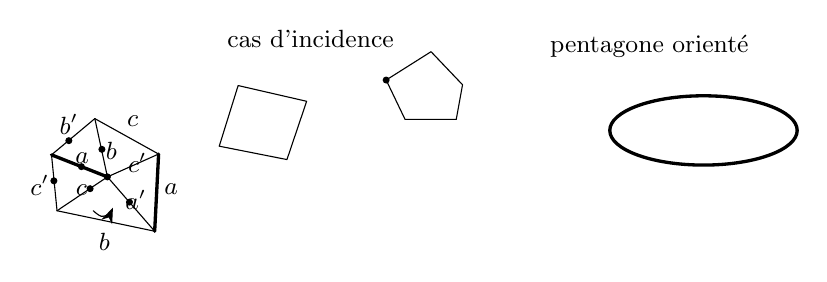
\begin{tikzpicture}[x=1mm,y=1mm,line cap=round,line join=round,font=\scriptsize]
\draw (11.2,-19.5) -- (19.3,-24);
\draw (18.8,-33.8) -- (6.4,-31.2);
\draw (6.4,-31.2) -- (5.7,-24.1);
\draw (5.7,-24.1) -- (11.2,-19.5);
\draw (12.8,-26.9) -- (11.2,-19.5);
\draw (12.8,-26.9) -- (6.4,-31.2);
\draw (12.8,-26.9) -- (19.3,-24);
\draw (12.8,-26.9) -- (18.8,-33.8);
\draw[very thick] (19.3,-24) -- (18.8,-33.8);
\draw[very thick] (12.8,-26.9) -- (5.7,-24.1);
\node[pt] at (7.9,-22.3) {};
\node[pt] at (6,-27.4) {};
\node[pt] at (12.1,-23.4) {};
\node[pt] at (9.5,-25.6) {};
\node[pt] at (10.6,-28.4) {};
\node[pt] at (15.6,-30.1) {};
\node[pt] at (12.8,-26.9) {};
\draw[-{Stealth[length=2mm]}] plot[smooth, tension=0.55] coordinates {(11,-31.2) (12,-31.9) (13,-31.6) (13.5,-30.8)};
\node[inner sep=1pt] at (7.9,-20.2) {\small $b'$};
\node[inner sep=1pt] at (16,-19.8) {\small $c$};
\node[inner sep=1pt] at (13.3,-23.6) {\small $b$};
\node[inner sep=1pt] at (9.6,-24.5) {\small $a$};
\node[inner sep=1pt] at (16.6,-25.1) {\small $c'$};
\node[inner sep=1pt] at (4.2,-28) {\small $c'$};
\node[inner sep=1pt] at (9.5,-28.6) {\small $c$};
\node[inner sep=1pt] at (20.9,-28.4) {\small $a$};
\node[inner sep=1pt] at (16.4,-29.8) {\small $a'$};
\node[inner sep=1pt] at (12.4,-35.2) {\small $b$};
\draw (29.4,-15.3) -- (38.1,-17.3) -- (35.6,-24.7) -- (27,-23) -- cycle;
\draw (48.2,-14.6) -- (53.9,-11) -- (57.9,-15.2) -- (57.1,-19.6) -- (50.6,-19.6) -- cycle;
\node[pt] at (48.2,-14.6) {};
\draw[very thick] (88.5,-21) ellipse[x radius=11.9, y radius=4.4];
\node[inner sep=1pt,anchor=west] at (27.6,-9.4) {\small cas d'incidence};
\node[inner sep=1pt,anchor=west] at (68.6,-10.3) {\small pentagone orienté};
\end{tikzpicture}
\end{document}
